%% chapter4_slides.tex
%% Beamer slides for Chapter 4: Relations of the Krasnosel'skiĭ-Mann Iteration
%% and the Operator Splitting Methods
%% "The Krasnosel'skiĭ-Mann Iterative Method: Recent Progress and Applications"
%% by Dong, Cho, He, Pardalos & Rassias (SpringerBriefs in Optimization, 2022)
%% Compiled with: pdflatex -interaction=nonstopmode chapter4_slides.tex  (twice)
\documentclass[aspectratio=169,10pt]{beamer}

\usetheme{Madrid}
\usecolortheme{seahorse}
\usefonttheme{professionalfonts}

%% ── Packages ──────────────────────────────────────────────────────────────
\usepackage{amsmath,amssymb,amsfonts}
\usepackage{mathtools}
\usepackage{graphicx}
\usepackage{booktabs}
\usepackage{xcolor}
\usepackage{listings}

\graphicspath{{figures/}}

%% ── Python listing style ─────────────────────────────────────────────────
\lstdefinestyle{pycode}{
  language=Python,
  basicstyle=\ttfamily\scriptsize,
  numbers=left,
  numberstyle=\tiny\color{gray},
  frame=single,
  backgroundcolor=\color{gray!7},
  keywordstyle=\color{blue!70!black}\bfseries,
  commentstyle=\color{green!50!black}\itshape,
  stringstyle=\color{orange!80!black},
  showstringspaces=false,
  breaklines=true,
  tabsize=2,
  xleftmargin=1.5em,
  framexleftmargin=1.5em,
  aboveskip=4pt,
  belowskip=4pt,
}
\lstset{style=pycode}

%% ── Metadata ─────────────────────────────────────────────────────────────
\title[KM Method -- Ch.4]{The Krasnosel'ski\u{i}-Mann Iterative Method}
\subtitle{Chapter 4: Relations to Operator Splitting Methods}
\author{Based on Dong, Cho, He, Pardalos \& Rassias}
\date{}

\setbeamertemplate{footline}[frame number]
\setbeamertemplate{navigation symbols}{}

%% ── Macros ────────────────────────────────────────────────────────────────
\newcommand{\Id}{\mathrm{Id}}
\newcommand{\prox}{\operatorname{prox}}
\newcommand{\Fix}{\operatorname{Fix}}
\newcommand{\zer}{\operatorname{zer}}
\newcommand{\ip}[2]{\langle #1, #2\rangle}
\newcommand{\bv}[1]{\mathbf{#1}}

\begin{document}

%% =========================================================================
\begin{frame}
  \titlepage
\end{frame}

%% =========================================================================
\begin{frame}{Where we are}
  \begin{itemize}
    \item \textbf{Chapter 2} gave us the vocabulary: nonexpansive / firmly nonexpansive / averaged operators, maximally monotone operators, subdifferentials, resolvents and proximal operators.
    \item \textbf{Chapter 3} gave us \emph{one} algorithm template, the Krasnosel'ski\u{i}--Mann (KM) iteration
    \[
      x_{n+1} = (1-\lambda_n)x_n + \lambda_n T x_n, \qquad T \text{ averaged (or nonexpansive)},
    \]
    and its convergence theory (weak convergence to a point of $\Fix(T)$ under mild conditions on $\{\lambda_n\}$).
    \item \textbf{Chapter 4's punchline:} gradient descent, the proximal point algorithm, forward-backward splitting, Douglas--Rachford, Davis--Yin, and primal-dual splitting are \emph{not} six different algorithms. They are \emph{one} algorithm -- ``iterate an averaged operator'' -- wearing six different operators $T$.
    \item Roadmap: 4.1 gradient descent, 4.2 proximal point, 4.3 splitting methods for $0\in A(x)+B(x)$ (or sums of several operators).
  \end{itemize}
\end{frame}

%% =========================================================================
\begin{frame}[allowframebreaks]{Notation you'll need / recap}
  \begin{block}{Averaged operator (recap from Ch.\ 2--3)}
    $T:\mathcal H\to\mathcal H$ is \emph{$\alpha$-averaged} ($\alpha\in(0,1)$) if there is a nonexpansive $R$ with $T=(1-\alpha)\Id+\alpha R$. Equivalently,
    \[
      \|Tx-Ty\|^2 \le \|x-y\|^2 - \frac{1-\alpha}{\alpha}\|(\Id-T)x-(\Id-T)y\|^2, \quad \forall x,y\in\mathcal H.
    \]
    Averaged operators are exactly the class of maps for which the KM iteration $x_{n+1}=(1-\lambda_n)x_n+\lambda_n Tx_n$ converges (weakly) to a fixed point, for suitable $\{\lambda_n\}$. \emph{Firmly nonexpansive} $=$ $\tfrac12$-averaged.
  \end{block}

  \begin{block}{Resolvent / proximal operator (recap)}
    For a maximally monotone $A:\mathcal H\rightrightarrows\mathcal H$ and $\gamma>0$, the \emph{resolvent} is
    \[
      J_{\gamma A} := (\Id+\gamma A)^{-1}.
    \]
    $J_{\gamma A}$ is single-valued, firmly nonexpansive, and $\Fix(J_{\gamma A})=\zer(A):=\{x: 0\in A(x)\}$. When $A=\partial f$ for $f\in\Gamma_0(\mathcal H)$ (proper, convex, lsc), $J_{\gamma\partial f}=\prox_{\gamma f}$, the \emph{proximal operator} of $f$. Special case: $f=\delta_C$ (indicator of a closed convex $C$) gives $\prox_{\gamma\delta_C}=P_C$, the metric projection onto $C$, \emph{for every} $\gamma>0$.
  \end{block}

  \begin{block}{Cocoercive operator (new name, old idea)}
    $B:\mathcal H\to\mathcal H$ is \emph{$\beta$-cocoercive} ($\beta>0$) if
    \[
      \ip{x-y}{Bx-By} \ge \beta\|Bx-By\|^2, \quad \forall x,y\in\mathcal H.
    \]
    By the Baillon--Haddad theorem, if $f$ is convex with $L$-Lipschitz gradient then $\nabla f$ is $\tfrac1L$-cocoercive -- this is exactly what makes an explicit (forward) gradient step behave well.
  \end{block}

  \framebreak

  \begin{block}{The monotone inclusion problem}
    Given a maximally monotone $A:\mathcal H\rightrightarrows\mathcal H$,
    \begin{equation*}
      \text{Find } x\in\mathcal H \text{ such that } 0\in A(x). \tag{4.3}
    \end{equation*}
    Minimizing $f\in\Gamma_0(\mathcal H)$ is the special case $A=\partial f$ (Fermat's rule): minimizers of $f$ $=$ zeros of $\partial f$ $=$ fixed points of $J_{\gamma\partial f}=\prox_{\gamma f}$.
  \end{block}

  \begin{block}{Why ``split'' at all?}
    Real problems often look like $0\in A(x)+B(x)$ (or a sum of several operators). In principle the proximal point algorithm could be applied directly to $A+B$ -- but $J_{\gamma(A+B)}$ is almost never computable in closed form, even when $J_{\gamma A}$ and $J_{\gamma B}$ (or a gradient step for $B$) individually are cheap. \emph{Operator splitting} means: build an iteration that only ever calls $J_{\gamma A}$, $J_{\gamma B}$, or $\nabla$(smooth part) \emph{separately}, never $J_{\gamma(A+B)}$ jointly. Typical division of labor: one piece is smooth/easy (cocoercive, take a gradient step), the other is nonsmooth/simple-to-prox (maximally monotone, take a resolvent step).
  \end{block}

  \begin{block}{Running example (carried over from earlier chapters)}
    $C=\{x\in\mathbb R^2:\|x\|\le 1\}$, the closed unit disk. For $p=(3,4)$, the projection is $P_C(p)=p/\|p\|=(0.6,0.8)$. Every algorithm in this chapter will, in some instantiation, reproduce exactly this point.
  \end{block}
\end{frame}

%% =========================================================================
\begin{frame}{The big picture: everything is an averaged-operator iteration}
  \centering
  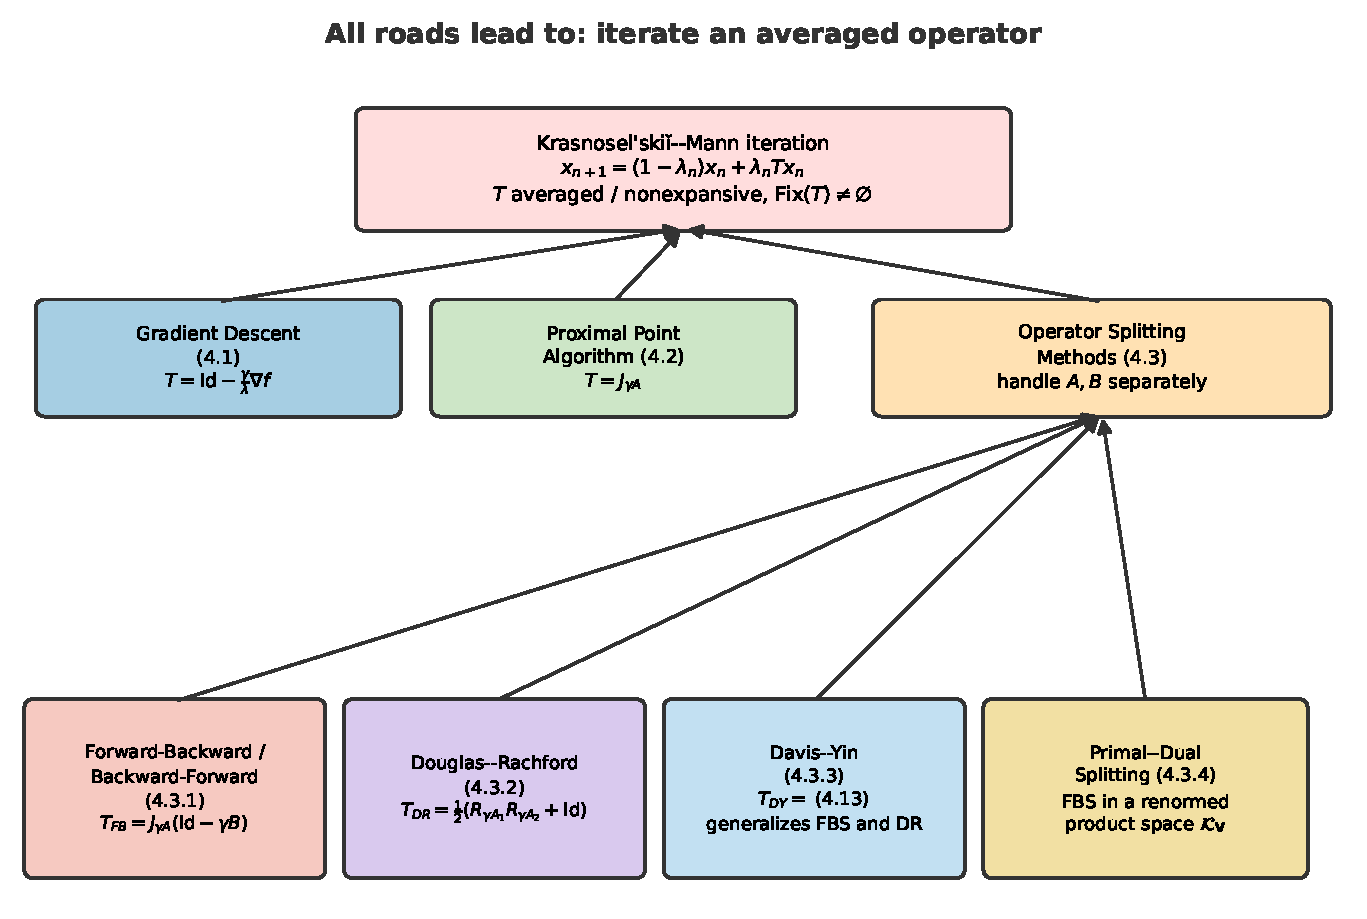
\includegraphics[height=5.4cm]{fig_family_tree.pdf}
\end{frame}

%% =========================================================================
\begin{frame}{4.1 Gradient descent -- why, and the formula}
  \begin{block}{Why would you want this?}
    You want to minimize a \emph{smooth} convex function $f:\mathcal H\to\mathbb R$ with $L$-Lipschitz gradient,
    \begin{equation*}
      \min_{x\in\mathcal H} f(x). \tag{4.1}
    \end{equation*}
    No constraints, no nonsmooth part -- the simplest possible instance of ``find a zero of a monotone operator'' ($A=\nabla f$, single-valued and monotone by convexity). The natural move: walk downhill along $-\nabla f$.
  \end{block}
  \begin{block}{Gradient Descent Algorithm}
    Let $f:\mathcal H\to\mathbb R$ be convex with $L$-Lipschitz gradient, $\{\gamma_n\}\subset(0,2/L)$. Choose $x_0\in\mathcal H$ arbitrarily and compute
    \begin{equation*}
      x_{n+1} = x_n - \gamma_n \nabla f(x_n), \qquad n\ge 0. \tag{4.2}
    \end{equation*}
    \emph{Symbols:} $\gamma_n$ is the step size; the range $(0,2/L)$ is exactly what makes this converge.
  \end{block}
\end{frame}

%% =========================================================================
\begin{frame}[allowframebreaks]{4.1 Derivation: GD \emph{is} a KM iteration}
  \begin{block}{Step 1 -- Baillon--Haddad}
    $\nabla f$ is $L$-Lipschitz $\iff$ $T:=\Id-\tfrac2L\nabla f$ is nonexpansive, and $\operatorname*{Argmin}_{x\in\mathcal H} f(x)=\Fix(T)$.
    (This is the Hilbert-space upgrade of ``convex $+$ Lipschitz gradient $\Rightarrow$ $\nabla f$ is cocoercive with constant $1/L$''.)
  \end{block}

  \begin{block}{Step 2 -- rewrite the GD step as a KM step}
    Start from (4.2) and insert a free parameter $\lambda_n\in(0,1]$:
    \[
      x_{n+1} = x_n - \gamma_n\nabla f(x_n)
              = (1-\lambda_n)x_n + \lambda_n\Big(x_n - \frac{\gamma_n}{\lambda_n}\nabla f(x_n)\Big).
    \]
    This is just algebra: $(1-\lambda_n)x_n+\lambda_n x_n = x_n$, and the leftover $-\gamma_n\nabla f(x_n)$ is absorbed by writing it as $\lambda_n\cdot(-\tfrac{\gamma_n}{\lambda_n}\nabla f(x_n))$.
  \end{block}

  \framebreak

  \begin{block}{Step 3 -- identify $T$ and check it is averaged}
    Define
    \[
      T := \Id - \frac{\gamma_n}{\lambda_n}\nabla f.
    \]
    Choosing $\lambda_n = \dfrac{\gamma_n L}{2}$ makes $\dfrac{\gamma_n}{\lambda_n}=\dfrac{2}{L}$, so $T=\Id-\tfrac2L\nabla f$ is \emph{exactly} the nonexpansive operator from Step 1. Then (4.2) is the KM iteration
    \[
      x_{n+1} = (1-\lambda_n)x_n + \lambda_n T x_n, \qquad \lambda_n=\frac{\gamma_n L}{2},
    \]
    and $\gamma_n\in(0,2/L) \iff \lambda_n\in(0,1)$, exactly the admissible KM relaxation range. Also $\Fix(T)=\operatorname*{Argmin} f$: the fixed points of $T$ are precisely the minimizers we wanted.
  \end{block}

  \begin{block}{Takeaway}
    Gradient descent is nothing but KM iteration of the nonexpansive operator $T=\Id-\tfrac2L\nabla f$, with the relaxation parameter $\lambda_n$ tied to the step size by $\lambda_n=\gamma_n L/2$. Small step size $\Leftrightarrow$ small (safe) relaxation.
  \end{block}
\end{frame}

%% =========================================================================
\begin{frame}{4.1 Running example: gradient descent on a quadratic}
  \begin{block}{Setup}
    $f(x)=\tfrac12\|x-p\|^2$ with $p=(3,4)$. Then $\nabla f(x)=x-p$ is $1$-Lipschitz ($L=1$), so $\gamma_n\in(0,2)$ is admissible. Take $\gamma_n\equiv 0.5$, $x_0=(0,0)$:
    \[
      x_{n+1} = x_n - 0.5\,(x_n-p) = 0.5\,x_n + 0.5\,p.
    \]
  \end{block}
  \begin{table}
    \centering
    \begin{tabular}{c c c}
      \toprule
      $n$ & $x_n$ & $\|x_n-p\|$ \\
      \midrule
      0 & $(0.000,\,0.000)$ & $5.000$ \\
      1 & $(1.500,\,2.000)$ & $2.500$ \\
      2 & $(2.250,\,3.000)$ & $1.250$ \\
      3 & $(2.625,\,3.500)$ & $0.625$ \\
      4 & $(2.8125,\,3.750)$ & $0.3125$ \\
      \bottomrule
    \end{tabular}
  \end{table}
  \begin{block}{Unconstrained minimizer}
    No constraint here, so GD converges to the unconstrained minimizer $p=(3,4)$ itself -- \emph{not} the disk-projection point $(0.6,0.8)$. We reuse this exact $f$ below (Section 4.3.1) once we add the disk constraint back in.
  \end{block}
\end{frame}

%% =========================================================================
\begin{frame}[fragile]{Python: gradient descent as a KM iteration}
\begin{lstlisting}
import numpy as np

p = np.array([3.0, 4.0])
L = 1.0                      # Lipschitz constant of grad f(x) = x - p
grad_f = lambda x: x - p

def gd_step(x, gamma):
    return x - gamma * grad_f(x)

def km_view_step(x, gamma):
    # same update, written as (1-lam)*x + lam*T(x), T = Id - (2/L) grad f
    lam = gamma * L / 2.0
    T = lambda z: z - (2.0 / L) * grad_f(z)
    return (1 - lam) * x + lam * T(x)

x = np.array([0.0, 0.0])
gamma = 0.5
for n in range(5):
    print(n, x, np.linalg.norm(x - p))
    x = gd_step(x, gamma)          # identical to km_view_step(x, gamma)
# -> converges geometrically to p = (3, 4)
\end{lstlisting}
\end{frame}

%% =========================================================================
\begin{frame}{4.2 Proximal point algorithm -- why, and the setup}
  \begin{block}{Why would you want this?}
    Gradient descent needs $f$ smooth. Many important problems are not: $f$ may be an indicator function, an $\ell_1$ norm, etc. Fermat's rule (Thm 2.1) says minimizing $f\in\Gamma_0(\mathcal H)$ is equivalent to finding a zero of $\partial f$. The proximal point algorithm solves the general monotone inclusion (4.3) for \emph{any} maximally monotone $A$ (not just subdifferentials), by repeatedly applying its resolvent.
  \end{block}
  \begin{block}{Proximal Point Algorithm}
    Let $A:\mathcal H\rightrightarrows\mathcal H$ be maximally monotone with $\zer(A)\ne\emptyset$, $\{\gamma_n\}\subset(0,+\infty)$, $\{\lambda_n\}\subset[0,2]$. Choose $x_0\in\mathcal H$ arbitrarily and compute
    \begin{equation*}
      x_{n+1} = (1-\lambda_n)x_n + \lambda_n J_{\gamma_n A}(x_n), \qquad n\ge 0. \tag{4.4}
    \end{equation*}
    With $\lambda_n\equiv 1$ this is Rockafellar's classical \emph{proximal point algorithm}; the general scheme (4.4) is the \emph{generalized proximal point algorithm} of Eckstein--Bertsekas.
  \end{block}
\end{frame}

%% =========================================================================
\begin{frame}{4.2 PPA \emph{is} already a KM iteration, verbatim}
  \begin{block}{Identify $T$}
    Take $T:=J_{\gamma_n A}$. Since $J_{\gamma_n A}$ is firmly nonexpansive (hence $\tfrac12$-averaged, in particular averaged), and
    \[
      \Fix(J_{\gamma_n A}) = \zer(A),
    \]
    the scheme (4.4) is \emph{literally} the KM iteration $x_{n+1}=(1-\lambda_n)x_n+\lambda_n T x_n$ with no algebraic massaging required at all -- unlike gradient descent, no re-parametrization step was needed.
  \end{block}
  \begin{block}{Why this matters}
    Because $T=J_{\gamma_n A}$ is already averaged for \emph{every} $\gamma_n>0$ and \emph{every} maximally monotone $A$, the KM convergence theory transfers immediately: (4.4) converges weakly to a point of $\zer(A)$ whenever $\{\lambda_n\}\subset[0,2]$ satisfies the usual divergence condition $\sum_n\lambda_n(2-\lambda_n)=\infty$.
  \end{block}
\end{frame}

%% =========================================================================
\begin{frame}{4.2 Running example: PPA reduces to the earlier projection}
  \begin{block}{Instantiation}
    Let $A=\partial\delta_C$, the subdifferential of the indicator of the unit disk $C$ (i.e.\ the normal cone operator $N_C$). Then, for \emph{every} $\gamma_n>0$,
    \[
      J_{\gamma_n A} = \prox_{\gamma_n\delta_C} = P_C
    \]
    -- the projection onto $C$, independent of $\gamma_n$! With $\lambda_n\equiv1$, (4.4) becomes the utterly familiar
    \[
      x_{n+1} = P_C(x_n).
    \]
  \end{block}
  \begin{block}{Numbers}
    Start at $x_0=p=(3,4)$ (outside $C$). Then $x_1=P_C(x_0)=(3,4)/5=(0.6,0.8)\in C$, and since $P_C(y)=y$ for $y\in C$, $x_n=(0.6,0.8)$ for every $n\ge1$: convergence in \emph{one step}. This is literally the running-example projection computation from earlier chapters, now seen as an instance of the proximal point algorithm with $A=\partial\delta_C$.
  \end{block}
\end{frame}

%% =========================================================================
\begin{frame}[fragile]{Python: proximal point algorithm for $A=\partial\delta_C$}
\begin{lstlisting}
import numpy as np

def P_C(x):                     # J_{gamma A} for A = subdifferential of
    n = np.linalg.norm(x)       # the indicator of the unit disk -- same
    return x / n if n > 1 else x  # for every gamma > 0

def ppa_step(x, lam=1.0):
    return (1 - lam) * x + lam * P_C(x)

x = np.array([3.0, 4.0])
for n in range(3):
    print(n, x)
    x = ppa_step(x)
# n=0: [3. 4.]
# n=1: [0.6 0.8]   <- Fix(P_C) reached: converged in one step
# n=2: [0.6 0.8]
\end{lstlisting}
\end{frame}

%% =========================================================================
\begin{frame}{4.3 The operator splitting methods -- setting the stage}
  \begin{block}{Problem 4.1: the general template}
    Let $B:\mathcal H\to\mathcal H$ be $\beta$-cocoercive for some $\beta>0$, $m\ge1$, and $A_i:\mathcal H\rightrightarrows\mathcal H$ maximally monotone for $i=1,\dots,m$. Find
    \begin{equation*}
      x\in\mathcal H \text{ such that } 0\in B(x)+\sum_{i=1}^m A_i(x). \tag{4.5}
    \end{equation*}
  \end{block}
  \begin{block}{Why not just run PPA on $A_1+\cdots+A_m+B$?}
    Even when every $J_{\gamma A_i}$ and $\nabla$ of the smooth piece are individually cheap, the resolvent of the \emph{sum} is essentially never available in closed form. \emph{Operator splitting methods} are iterations that only ever call the resolvents/gradients of the pieces \emph{separately}. The rest of Section 4.3 exhibits four such methods, all of which turn out to be KM iterations for a cleverly built averaged operator $T$.
  \end{block}
\end{frame}

%% =========================================================================
\begin{frame}[allowframebreaks]{4.3.1 Forward-backward splitting -- why, and the operator}
  \begin{block}{Problem 4.1.1 ($m=1$)}
    Find $x\in\mathcal H$ such that $0\in(A+B)(x)$, where (a) $A$ is maximally monotone, (b) $B$ is $\beta$-cocoercive for some $\beta>0$, (c) $\zer(A+B)\ne\emptyset$. (4.6)
  \end{block}
  \begin{block}{Why would you want this?}
    $B$ smooth/cocoercive $\Rightarrow$ an explicit \emph{forward} (gradient-like) step is cheap; $A$ possibly nonsmooth $\Rightarrow$ only its resolvent (an \emph{implicit}/\emph{backward} step) is cheap. Forward-backward splitting alternates the two: take a forward step to ``deal with'' $B$, then a backward step to ``deal with'' $A$.
  \end{block}
  \begin{block}{Lemma 4.1 -- the averaged operator}
    Let $\gamma\in(0,2\beta)$ and define
    \[
      T_{FB} := J_{\gamma A}(\Id-\gamma B).
    \]
    Then (1) $T_{FB}$ is $\dfrac{2\beta}{4\beta-\gamma}$-averaged; (2) $\zer(A+B)=\Fix(T_{FB})$.
  \end{block}

  \framebreak

  \begin{block}{The forward-backward splitting method}
    Let $\gamma\in(0,2\beta)$, $\{\lambda_n\}\subset\big[0,\tfrac{4\beta-\gamma}{2\beta}\big]$ with $\sum_n\lambda_n\big(\tfrac{4\beta-\gamma}{2\beta}-\lambda_n\big)=\infty$. Choose $x_0\in\mathcal H$ and iterate
    \begin{equation*}
      x_{n+1} = (1-\lambda_n)x_n + \lambda_n T_{FB}x_n, \qquad n\ge0. \tag{4.7}
    \end{equation*}
    Unwound: $x_{n+1}=(1-\lambda_n)x_n+\lambda_n J_{\gamma A}\big(x_n-\gamma B(x_n)\big)$ -- an explicit gradient-type step on $B$, then an implicit resolvent step on $A$, then a KM relaxation.
  \end{block}
  \begin{block}{(B) Backward-forward splitting -- Lemma 4.2}
    Swap the order: $T_{BF}:=(\Id-\gamma B)J_{\gamma A}$ is also $\dfrac{2\beta}{4\beta-\gamma}$-averaged, with $\zer(A_\gamma+B_{-\gamma})=\Fix(T_{BF})$ (a shifted version of the same zero set). The iteration
    \begin{equation*}
      x_{n+1} = (1-\lambda_n)x_n + \lambda_n T_{BF}x_n \tag{4.8}
    \end{equation*}
    does the resolvent step \emph{first}, the gradient step \emph{second}. It arises from time-discretizing the regularized Newton method for maximally monotone operators, and shares the same basic building blocks as FBS, just organized differently.
  \end{block}
\end{frame}

%% =========================================================================
\begin{frame}{4.3.1 Running example: FBS on quadratic $+$ disk indicator}
  \begin{block}{Instantiation}
    $f(x)=\tfrac12\|x-p\|^2$ (smooth, $B=\nabla f$, $1$-cocoercive, $p=(3,4)$), $g=\delta_C$ (nonsmooth indicator of the unit disk, $A=\partial g$, $J_{\gamma A}=P_C$ for all $\gamma$). With $\gamma=0.5\in(0,2)$, $\lambda_n\equiv1$, $x_0=(-2,3)$:
    \[
      x_{n+1} = P_C\big(x_n - 0.5(x_n-p)\big).
    \]
  \end{block}
  \begin{table}
    \centering\small
    \begin{tabular}{c c c}
      \toprule
      $n$ & $x_n$ & $\|x_n-(0.6,0.8)\|$ \\
      \midrule
      0 & $(-2.000,\,3.000)$ & $3.406$ \\
      1 & $(0.141,\,0.990)$ & $0.496$ \\
      2 & $(0.533,\,0.846)$ & $0.082$ \\
      3 & $(0.589,\,0.808)$ & $0.014$ \\
      6 & $(0.5999,\,0.80004)$ & $6.3\times10^{-5}$ \\
      \bottomrule
    \end{tabular}
  \end{table}
  Converges to the \emph{same} point $(0.6,0.8)=P_C(p)$ as the earlier running example -- now obtained by \emph{splitting} $f+\delta_C$ instead of directly projecting.
\end{frame}

%% =========================================================================
\begin{frame}{4.3.1 The iterates, geometrically and in error}
  \centering
  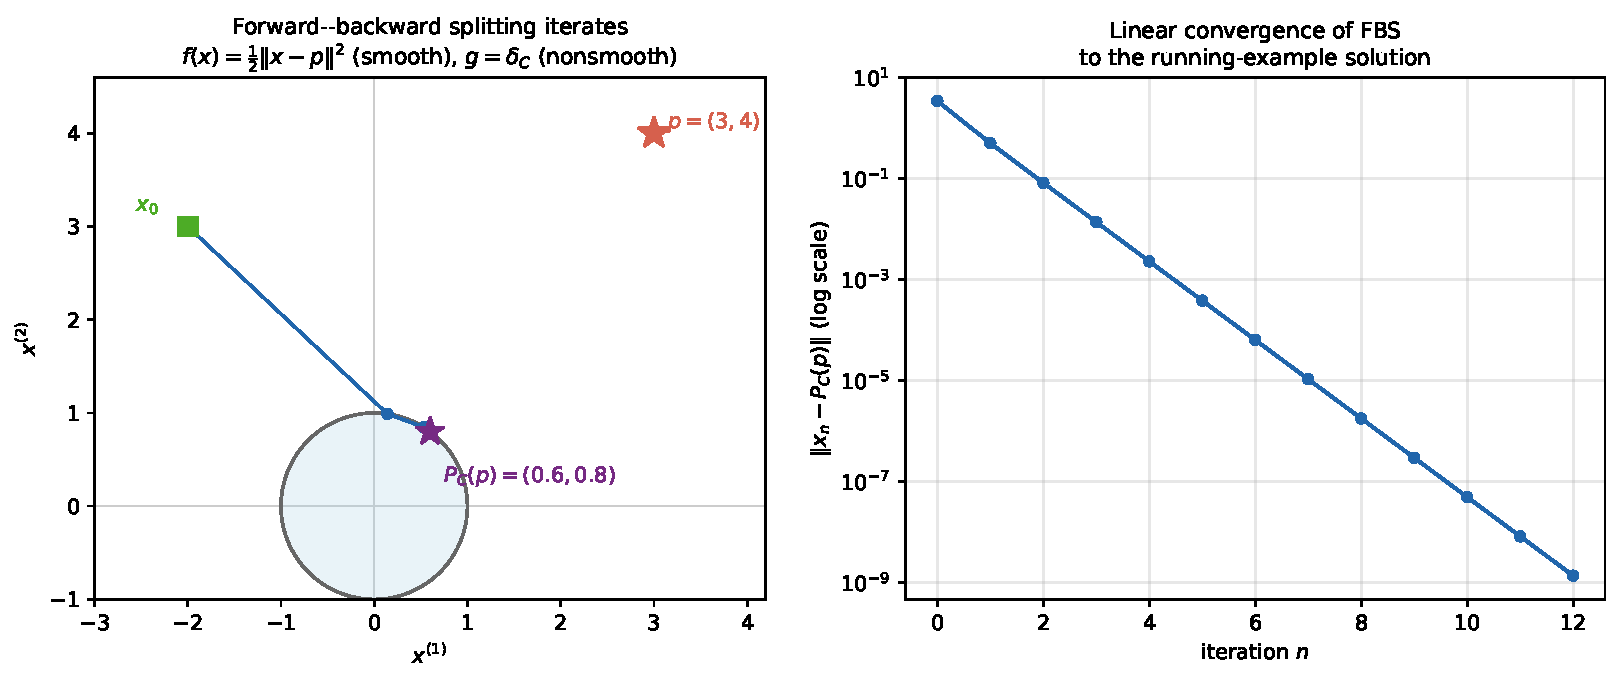
\includegraphics[width=\linewidth]{fig_fbs_convergence.pdf}
\end{frame}

%% =========================================================================
\begin{frame}{4.3.1 Three KM instances, one running example}
  \centering
  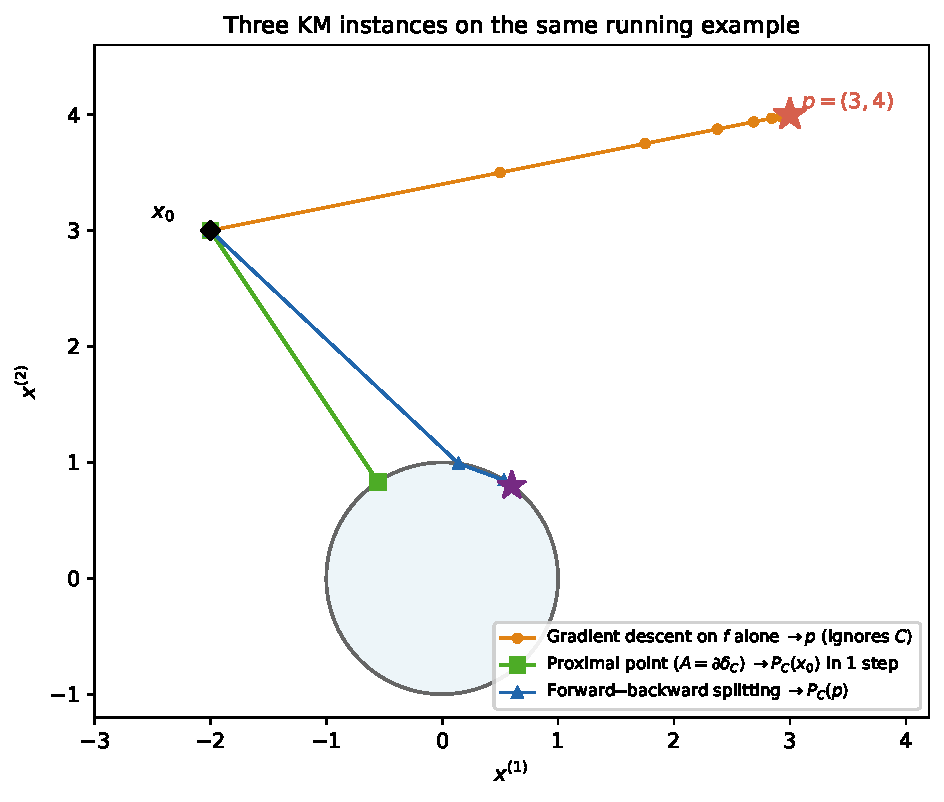
\includegraphics[width=0.62\linewidth]{fig_three_methods_compare.pdf}\\
  {\footnotesize Gradient descent ignores the constraint; PPA on $\partial\delta_C$ jumps straight to $P_C(x_0)$; FBS on $f+\delta_C$ converges to $P_C(p)$.}
\end{frame}

%% =========================================================================
\begin{frame}[fragile]{Python: forward-backward splitting}
\begin{lstlisting}
import numpy as np

p = np.array([3.0, 4.0])
grad_f = lambda x: x - p        # B = grad f, 1-cocoercive (L = 1)

def P_C(x):                     # J_{gamma A}, A = subdifferential of delta_C
    n = np.linalg.norm(x)
    return x / n if n > 1 else x

def fbs_step(x, gamma=0.5):
    y = x - gamma * grad_f(x)   # forward step on B
    return P_C(y)               # backward step on A

x = np.array([-2.0, 3.0])
target = np.array([0.6, 0.8])
for n in range(7):
    print(n, x, np.linalg.norm(x - target))
    x = fbs_step(x)
# -> converges linearly to (0.6, 0.8) = P_C(p)
\end{lstlisting}
\end{frame}

%% =========================================================================
\begin{frame}[allowframebreaks]{4.3.2 Douglas--Rachford splitting -- why, and the operator}
  \begin{block}{Problem 4.1.2 ($B=0$, $m=2$)}
    Find $x\in\mathcal H$ such that $0\in(A_1+A_2)(x)$, where $A_1,A_2$ are maximally monotone and $\zer(A_1+A_2)\ne\emptyset$. (4.9)
  \end{block}
  \begin{block}{Why would you want this?}
    FBS needed one of the two pieces to be \emph{cocoercive} (smooth). Douglas--Rachford drops that requirement entirely: both $A_1,A_2$ may be nonsmooth maximally monotone operators (e.g.\ two normal-cone operators for a convex-feasibility problem, or two nonsmooth regularizers). All you need are the two resolvents.
  \end{block}
  \begin{block}{Reflected resolvent (recap)}
    Write $R_{\gamma A}:=2J_{\gamma A}-\Id$ (the reflection through the resolvent). $R_{\gamma A}$ is nonexpansive whenever $A$ is maximally monotone, because $J_{\gamma A}$ is firmly nonexpansive.
  \end{block}

  \framebreak

  \begin{block}{Lemma 4.3 -- the averaged operator}
    Let $\gamma>0$ and define
    \[
      T_{DR} := \tfrac12\big(R_{\gamma A_1}R_{\gamma A_2}+\Id\big).
    \]
    Then: (1) $R_{\gamma A_1}R_{\gamma A_2}$ is nonexpansive; (2) $T_{DR}=J_{\gamma A_1}(2J_{\gamma A_2}-\Id)-J_{\gamma A_2}+\Id$ is firmly nonexpansive (i.e.\ $\tfrac12$-averaged -- being the average of a nonexpansive map and $\Id$ is automatic); (3) $\zer(A_1+A_2)=J_{\gamma A_2}(\Fix(T_{DR}))$.
  \end{block}
  \begin{block}{The Douglas--Rachford splitting method}
    Let $\gamma>0$, $\{\lambda_n\}\subset[0,2]$ with $\sum_n\lambda_n(2-\lambda_n)=\infty$. Choose $x_0\in\mathcal H$; for each $n\ge0$,
    \begin{equation*}
      \begin{cases}
        y_n = J_{\gamma A_2}x_n, \\
        z_n = J_{\gamma A_1}(2y_n-x_n), \\
        x_{n+1} = x_n+\lambda_n(z_n-y_n),
      \end{cases} \tag{4.10}
    \end{equation*}
    which is exactly the KM iteration $x_{n+1}=(1-\lambda_n)x_n+\lambda_n T_{DR}(x_n)$. (4.11)
  \end{block}

  \framebreak

  \begin{block}{Remarks}
    \begin{itemize}
      \item $\lambda_n\equiv 2$ recovers the \emph{Peaceman--Rachford} splitting method.
      \item The solution to (4.9) is recovered as $y=J_{\gamma A_2}(x^\star)$ where $x^\star\in\Fix(T_{DR})$ -- note the fixed point of $T_{DR}$ is generally \emph{not itself} the solution, only its image under $J_{\gamma A_2}$ is.
      \item Douglas--Rachford is, in turn, a special case of the proximal point algorithm (via a product-space trick), and is closely related to ADMM and the primal-dual hybrid gradient method.
    \end{itemize}
  \end{block}
\end{frame}

%% =========================================================================
\begin{frame}{4.3.2 Running example (extended): two-disk feasibility}
  \begin{block}{A natural extension of the running example}
    Let $A_1=N_{C_1}$, $A_2=N_{C_2}$ (normal cones $=$ subdifferentials of indicators), with $C_1$ the unit disk centered at the origin (our familiar $C$) and $C_2$ the unit disk centered at $(1,0)$. Then $J_{\gamma A_i}=P_{C_i}$ for every $\gamma$, and $\zer(A_1+A_2)$ is exactly the lens-shaped intersection $C_1\cap C_2$ -- Douglas--Rachford becomes a \emph{projections onto convex sets} method for convex feasibility.
  \end{block}
  \begin{block}{Numbers ($\gamma=1$, $\lambda_n\equiv1$, $x_0=(2,2)$)}
    \centering\small
    \begin{tabular}{c c c}
      \toprule
      $n$ & $x_n$ & $y_n=P_{C_2}(x_n)$ \\
      \midrule
      0 & $(2.000,\,2.000)$ & $(1.447,\,0.894)$ \\
      1 & $(1.447,\,0.894)$ & $(1.447,\,0.894)$ \\
      2 & $(0.851,\,0.526)$ & $(0.851,\,0.526)$ \\
      $\ge3$ & $(0.851,\,0.526)$ & $(0.851,\,0.526)$ \\
      \bottomrule
    \end{tabular}
  \end{block}
  The limit $(0.851,0.526)$ lies on $\partial C_1$ and strictly inside $C_2$: a genuine point of $C_1\cap C_2$, found without ever forming $J_{\gamma(A_1+A_2)}$ directly.
\end{frame}

%% =========================================================================
\begin{frame}[fragile]{Python: Douglas--Rachford splitting}
\begin{lstlisting}
import numpy as np

c1, c2 = np.array([0.0, 0.0]), np.array([1.0, 0.0])   # centers, radius 1

def P_disk(x, c, r=1.0):
    d = x - c
    n = np.linalg.norm(d)
    return c + d / n * r if n > r else x

def dr_step(x, gamma=1.0, lam=1.0):
    y = P_disk(x, c2)              # J_{gamma A2}
    z = P_disk(2 * y - x, c1)      # J_{gamma A1}(2y - x)
    return x + lam * (z - y)

x = np.array([2.0, 2.0])
for n in range(4):
    y = P_disk(x, c2)
    print(n, "x=", x, " feasible pt y=", y)
    x = dr_step(x)
# -> y converges to (0.851, 0.526) in C1 cap C2
\end{lstlisting}
\end{frame}

%% =========================================================================
\begin{frame}[allowframebreaks]{4.3.3 Davis--Yin splitting -- why, and the operator}
  \begin{block}{Problem 4.1.3 ($m=2$, with a cocoercive piece back)}
    Find $x\in\mathcal H$ such that $0\in(A_1+A_2+B)(x)$: $A_1,A_2$ maximally monotone, $B$ $\beta$-cocoercive, $\zer(A_1+A_2+B)\ne\emptyset$. (4.12)
  \end{block}
  \begin{block}{Why would you want this?}
    Real objectives often have \emph{three} pieces: two nonsmooth regularizers/constraints ($A_1,A_2$) plus one smooth data-fitting term ($B$). Neither FBS (built for one nonsmooth $+$ one smooth piece) nor Douglas--Rachford (built for two nonsmooth pieces, no smooth part) directly applies. Davis--Yin splitting handles all three simultaneously, and specializes to FBS ($A_2=0$) or to Douglas--Rachford ($B=0$).
  \end{block}
  \begin{block}{Lemma 4.4 -- the averaged operator}
    Let $\gamma\in(0,2\beta)$ and define
    \begin{equation*}
      T_{DY} := J_{\gamma A_1}\big(2J_{\gamma A_2}-\Id-\gamma BJ_{\gamma A_2}\big) + \Id - J_{\gamma A_2}. \tag{4.13}
    \end{equation*}
    Then $T_{DY}$ is $\dfrac{2\beta}{4\beta-\gamma}$-averaged, and $\zer(A_1+A_2+B)=J_{\gamma A_2}(\Fix(T_{DY}))$.
  \end{block}

  \framebreak

  \begin{block}{The Davis--Yin splitting method}
    Let $\gamma\in(0,2\beta)$, $\{\lambda_n\}\subset\big[0,\tfrac{4\beta-\gamma}{2\beta}\big]$ with $\sum_n\lambda_n\big(\tfrac{4\beta-\gamma}{2\beta}-\lambda_n\big)=\infty$. Choose $x_0\in\mathcal H$; for each $n\ge0$,
    \begin{equation*}
      \begin{cases}
        y_n = J_{\gamma A_2}x_n, \\
        z_n = J_{\gamma A_1}(2y_n-x_n-\gamma B y_n), \\
        x_{n+1} = x_n+\lambda_n(z_n-y_n),
      \end{cases} \tag{4.14}
    \end{equation*}
    exactly the KM iteration $x_{n+1}=(1-\lambda_n)x_n+\lambda_n T_{DY}(x_n)$. (4.15)
  \end{block}
  \begin{block}{Spot the pattern}
    (4.14) is (4.10) with one extra term $-\gamma B y_n$ inserted into the middle line. Setting $A_2\equiv0$ (so $J_{\gamma A_2}=\Id$, $y_n=x_n$) collapses (4.14) to FBS (4.7); setting $B\equiv0$ collapses it to Douglas--Rachford (4.10). Davis--Yin genuinely \emph{is} the common generalization.
  \end{block}
\end{frame}

%% =========================================================================
\begin{frame}{4.3.3 Running example: adding a smooth term to two-disk feasibility}
  \begin{block}{Instantiation}
    Same $C_1,C_2$ as before ($A_1=N_{C_1}$, $A_2=N_{C_2}$), now with $B=\Id$ (gradient of $f(x)=\tfrac12\|x\|^2$, $1$-cocoercive). This solves
    \[
      \min_{x\in C_1\cap C_2} \tfrac12\|x\|^2 \iff 0\in \big(N_{C_1}+N_{C_2}+\Id\big)(x):
    \]
    the \emph{minimum-norm} point of the feasible lens $C_1\cap C_2$, not just \emph{some} feasible point.
  \end{block}
  \begin{block}{Numbers ($\gamma=1$, $\lambda_n\equiv1$, $x_0=(2,2)$)}
    \centering\small
    \begin{tabular}{c c}
      \toprule
      $n$ & $y_n=J_{\gamma A_2}(x_n)$ \\
      \midrule
      0 & $(1.447,\,0.894)$ \\
      1 & $(0.106,\,0.211)$ \\
      $\ge2$ & $(0.000,\,0.000)$ \\
      \bottomrule
    \end{tabular}
  \end{block}
  Since the origin lies \emph{on} $\partial C_2$ and at the center of $C_1$, it is feasible and clearly of minimal norm -- Davis--Yin finds it exactly, whereas plain Douglas--Rachford above found the different feasible point $(0.851,0.526)$: the extra cocoercive term $B$ changes \emph{which} point of $C_1\cap C_2$ we converge to.
\end{frame}

%% =========================================================================
\begin{frame}[fragile]{Python: Davis--Yin splitting}
\begin{lstlisting}
import numpy as np

c1, c2 = np.array([0.0, 0.0]), np.array([1.0, 0.0])

def P_disk(x, c, r=1.0):
    d = x - c
    n = np.linalg.norm(d)
    return c + d / n * r if n > r else x

B = lambda x: x                 # grad of f(x) = 1/2 ||x||^2, 1-cocoercive

def dy_step(x, gamma=1.0, lam=1.0):
    y = P_disk(x, c2)                      # J_{gamma A2}
    z = P_disk(2 * y - x - gamma * B(y), c1)  # J_{gamma A1}(...)
    return x + lam * (z - y)

x = np.array([2.0, 2.0])
for n in range(4):
    y = P_disk(x, c2)
    print(n, "min-norm feasible pt y=", y)
    x = dy_step(x)
# -> y converges to (0, 0): the minimum-norm point of C1 cap C2
\end{lstlisting}
\end{frame}

%% =========================================================================
\begin{frame}[allowframebreaks]{4.3.4 Primal-dual splitting -- why, and the problem}
  \begin{block}{Why would you want this?}
    So far every splitting method needed \emph{direct access} to each operator. But composite problems often involve a linear map, e.g.\ minimizing $f(x)+g(Lx)$ for a bounded linear $L$ (think: total-variation regularization, constrained optimization $Lx=b$). Applying a resolvent to ``$g\circ L$'' directly is typically intractable even when $\prox_g$ is easy. Primal-dual splitting handles $A,B,C,D,L$ \emph{all separately}, paying for $L$ and $L^*$ (its adjoint) only through matrix-vector products.
  \end{block}
  \begin{block}{Problem 4.1.4}
    Let $\mathcal H,\mathcal G$ be real Hilbert spaces with (a) $A$ maximally monotone, $B$ $\beta_B$-cocoercive on $\mathcal H$; (b) $C$ maximally monotone, $D$ $\beta_D$-strongly monotone on $\mathcal H$; (c) $L:\mathcal H\to\mathcal G$ bounded linear. The \emph{primal monotone inclusion} is
    \begin{equation*}
      \text{Find } x\in\mathcal H:\ 0\in(A+B)(x)+L^*\big((C\,\square\,D)(Lx)\big), \tag{4.16}
    \end{equation*}
    where $C\,\square\,D:=(C^{-1}+D^{-1})^{-1}$ is the \emph{parallel sum}. The \emph{dual problem} is
    \begin{equation*}
      \text{Find } v\in\mathcal G:\ (\exists\, x\in\mathcal H)\ \begin{cases} 0\in(A+B)(x)+L^*v, \\ 0\in(C^{-1}+D^{-1})(v)-Lx. \end{cases} \tag{4.17}
    \end{equation*}
    Assume both solution sets $\mathcal P$ (primal), $\mathcal D$ (dual) are nonempty.
  \end{block}

  \framebreak

  \begin{block}{(A) The primal-dual splitting iteration}
    Choose $\gamma_A,\gamma_C>0$ with
    \begin{equation*}
      2\min\{\beta_B,\beta_D\}\min\Big\{\frac1{\gamma_A},\frac1{\gamma_C}\Big\}\Big(1-\sqrt{\gamma_A\gamma_C\|L\|^2}\Big) > 1. \tag{4.18}
    \end{equation*}
    Choose $x_0\in\mathcal H$, $v_0\in\mathcal G$; for each $n\ge0$,
    \begin{equation*}
      \begin{cases}
        x_{n+1} = J_{\gamma_A A}\big(x_n-\gamma_A B(x_n)-\gamma_A L^*v_n\big), \\
        \bar x_{n+1} = 2x_{n+1}-x_n, \\
        v_{n+1} = J_{\gamma_C C^{-1}}\big(v_n-\gamma_C D^{-1}(v_n)+\gamma_C L\bar x_{n+1}\big).
      \end{cases} \tag{4.19}
    \end{equation*}
    Reading it: a forward-backward step in $x$ (treating $L^*v_n$ as a fixed forcing term), an over-relaxation $\bar x_{n+1}$, then a forward-backward step in $v$ using the fresh $\bar x_{n+1}$ -- primal and dual variables updated in an alternating, coupled fashion.
  \end{block}

  \framebreak

  \begin{block}{(B) The fixed point reformulation}
    Stack primal and dual variables $z_n:=\binom{x_n}{v_n}$ in the product space $\mathcal K=\mathcal H\times\mathcal G$, and define block operators
    \begin{equation*}
      \bv{A} := \begin{bmatrix} A & L^* \\ -L & C^{-1} \end{bmatrix}\!, \
      \bv{B} := \begin{bmatrix} B & 0 \\ 0 & D^{-1} \end{bmatrix}\!, \
      \bv{V} := \begin{bmatrix} \Id_{\mathcal H}/\gamma_A & -L^* \\ -L & \Id_{\mathcal G}/\gamma_C \end{bmatrix}\!. \tag{4.21}
    \end{equation*}
    Then (4.19) is equivalent to $-\bv{B}(z_n)\in\bv{A}(z_{n+1})+\bv{V}(z_{n+1}-z_n)$ (Eq.\ 4.20), i.e.
    \begin{equation*}
      z_{n+1} = (\bv{V}+\bv{A})^{-1}(\bv{V}-\bv{B})(z_n) = (\Id+\bv{V}^{-1}\bv{A})^{-1}(\Id-\bv{V}^{-1}\bv{B})(z_n). \tag{4.22}
    \end{equation*}
  \end{block}
  \begin{block}{The punchline}
    $\bv{A}$ is maximally monotone, $\bv{V}^{-1}\bv{B}$ is $\eta\rho$-cocoercive with $\eta=\min\{\beta_B,\beta_D\}$ and $\bv{V}$'s positivity constant $\rho$ set exactly by condition (4.18). So (4.22) is \emph{forward-backward splitting, Section 4.3.1's $T_{FB}$}, run inside the Hilbert space $\mathcal K_{\bv V}$ induced by the self-adjoint positive-definite $\bv{V}$ (i.e.\ with inner product $\ip{\cdot}{\cdot}_{\bv V}$ instead of the usual one). The fixed-point operator $\bv{T}_{FB}=J_{\bv{V}^{-1}\bv{A}}(\Id-\bv{V}^{-1}\bv{B})$ is $\dfrac{2\eta\rho}{4\eta\rho-1}$-averaged: same averaged-operator template, just in a re-normed product space.
  \end{block}
\end{frame}

%% =========================================================================
\begin{frame}{Summary: the unifying table}
  \centering\footnotesize
  \begin{tabular}{p{2.6cm} p{4.6cm} p{2.3cm} p{2.7cm}}
    \toprule
    \textbf{Method} & \textbf{Operator $T$} & \textbf{Averaging} & \textbf{$\Fix(T)$} \\
    \midrule
    Gradient descent & $\Id-\tfrac2L\nabla f$ & nonexpansive & $\operatorname*{Argmin} f$ \\
    Proximal point & $J_{\gamma A}$ & $\tfrac12$ (firmly n.e.) & $\zer(A)$ \\
    Forward-backward & $J_{\gamma A}(\Id-\gamma B)$ & $\tfrac{2\beta}{4\beta-\gamma}$ & $J_{\gamma A}^{-1}$-related to $\zer(A+B)$ \\
    Douglas--Rachford & $\tfrac12(R_{\gamma A_1}R_{\gamma A_2}+\Id)$ & $\tfrac12$ (firmly n.e.) & maps via $J_{\gamma A_2}$ to $\zer(A_1+A_2)$ \\
    Davis--Yin & $T_{DY}$, Eq.\ (4.13) & $\tfrac{2\beta}{4\beta-\gamma}$ & maps via $J_{\gamma A_2}$ to $\zer(A_1+A_2+B)$ \\
    Primal-dual & FBS's $T_{FB}$ in $\mathcal K_{\bv V}$ & $\tfrac{2\eta\rho}{4\eta\rho-1}$ & product-space solution $(x^\star,v^\star)$ \\
    \bottomrule
  \end{tabular}
  \vspace{0.4cm}
  \begin{block}{Every row: $x_{n+1}=(1-\lambda_n)x_n+\lambda_n Tx_n$}
    Different $T$, same convergence machinery from Chapter 3. This is exactly why the KM iteration -- with its built-in relaxation parameters $\lambda_n$ -- is the natural language for \emph{designing} operator splitting methods, not just analyzing them after the fact.
  \end{block}
\end{frame}

%% =========================================================================
\begin{frame}{Takeaways \& what's next}
  \begin{itemize}
    \item Gradient descent, the proximal point algorithm, forward-/backward-forward splitting, Douglas--Rachford, Davis--Yin, and primal-dual splitting all reduce to KM iteration $x_{n+1}=(1-\lambda_n)x_n+\lambda_nTx_n$ for a suitable averaged $T$.
    \item The running example (projection onto the unit disk) threaded through every method: gradient descent (unconstrained quadratic), proximal point (single resolvent $=P_C$), forward-backward (quadratic $+$ indicator), and its two-disk extension for Douglas--Rachford and Davis--Yin.
    \item The recurring design trick: split a hard joint resolvent $J_{\gamma(A+B+\cdots)}$ into cheap pieces ($J_{\gamma A_i}$, gradient steps), then package the resulting map as one averaged operator so that KM theory applies verbatim.
    \item \textbf{Next (Chapter 5):} accelerating the KM iteration itself via inertial (heavy-ball-type) extrapolation terms -- squeezing faster convergence out of the very same averaged-operator framework.
  \end{itemize}
\end{frame}

\end{document}
